% !TEX TS-program = pdfLaTeX+shellescape
% !TEX encoding = UTF-8 Unicode

\documentclass[class=beamer,tikz]{standalone}
\setbeamertemplate{navigation symbols}{} % For delete the navigation symbols
\usefonttheme{professionalfonts}
\usepackage{luatexja}
% \usepackage{pgfplots}
% \pgfplotsset{compat=1.17}

\usepackage{colortbl,array,xcolor}
\usepackage{amsmath,amsfonts}
\usepackage{bm}

\begin{document}
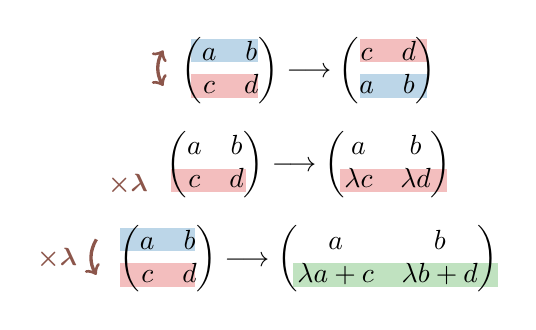
\begin{tikzpicture}
    \definecolor{tab_red}{HTML}{d62728}
    \definecolor{tab_blue}{HTML}{1f77b4}
    \definecolor{tab_green}{HTML}{2ca02c}
    \definecolor{tab_brown}{HTML}{8c564b}
    %\draw[help lines] (0,0) grid (10,6);
    \path[fill=tab_blue!30] (3.50,3.50) rectangle (4.35,3.80);
    \path[fill=tab_red!30] (3.50,3.05) rectangle (4.35,3.35);
    \path[fill=tab_red!30] (5.65,3.50) rectangle (6.50,3.80);
    \path[fill=tab_blue!30] (5.65,3.05) rectangle (6.50,3.35);
    \path[fill=tab_red!30] (3.25,1.85) rectangle (4.20,2.15);
    \path[fill=tab_red!30] (5.40,1.85) rectangle (6.75,2.15);
    \path[fill=tab_blue!30] (2.60,1.10) rectangle (3.55,1.40);
    \path[fill=tab_red!30] (2.60,0.65) rectangle (3.55,0.95);
    \path[fill=tab_green!30] (4.80,0.65) rectangle (7.40,0.95);

    \node (change1) at (5,3.4) {
        $\begin{pmatrix}
            a & b \cr 
            c & d
        \end{pmatrix}  
        \longrightarrow \begin{pmatrix}
            c & d \cr 
            a & b 
        \end{pmatrix}$
    };
    \node (change2) at (5,2.2) {
        $\begin{pmatrix}
            a & b \cr 
            c & d
        \end{pmatrix} \longrightarrow \begin{pmatrix}
            a & b \cr 
            \lambda c & \lambda d 
        \end{pmatrix}$
    };
    \node (change3) at (5,1) {
        $\begin{pmatrix}
            a & b \cr 
            c & d
        \end{pmatrix} \longrightarrow \begin{pmatrix}
            a & b \cr 
            \lambda a + c & \lambda b + d 
        \end{pmatrix}$
    };
    \draw[color=tab_brown, very thick, <->] (3.15,3.65) to [out=240, in=120] (3.15,3.2);
    \node[color=tab_brown] at (2.70,1.95) {\small$\bm{\times\lambda}$};
    \draw[color=tab_brown, very thick, ->] (2.30,1.25) to [out=240, in=120] (2.30,0.8);
    \node[color=tab_brown] at (1.80,1.00) {\small$\bm{\times\lambda}$};
    
\end{tikzpicture}
\end{document}